\chapter{Work done}
\label{chapter:work_done}

\section{Metadata Analysis}

Um dos desafios enfrentados na luta contra ataques de phishing é a obsolescência dos datasets atualmente disponíveis. Muitos desses conjuntos de dados não refletem as técnicas e estratégias mais recentes utilizadas, tornando as ferramentas de detecção menos eficazes contra novos ataques. Para superar este problema, propôs-se a criação de um dataset sintético que incorpore as características dos ataques de phishing mais recentes.

Inicialmente, foi necessário recolher uma coleção de e-mails de phishing reais e recentes. Esses e-mails servem como base para entender as tendências atuais e as técnicas utilizadas pelos phishers. A análise dos metadados desses e-mails é crucial, pois oferece insights sobre padrões comuns que podem ser replicados de forma sintética para enriquecer o dataset. Os metadados recolhidos incluem, mas não se limitam a, o endereço de e-mail do remetente, o destinatário, o assunto do e-mail, a data de envio, além de outros campos que podem revelar padrões de comportamento dos atacantes. Essas informações são essenciais para criar um modelo realista de headers de e-mail.

Com o auxilio de bibliotecas de python, desenvolveu-se um script capaz de gerar headers de e-mail fictícios. Este script utiliza os metadados extraídos dos e-mails reais como referência para criar headers convincentes que imitam autenticamente os utilizados em campanhas de phishing. A geração de headers fictícios inclui a manipulação cuidadosa de campos como o remetente, o destinatário e a data, de modo que os e-mails sintéticos pareçam plausíveis aos sistemas de detecção baseados em análise de metadados.

No final o objetivo é possuir um dataset de e-mails de phishing sintéticos que possam ser utilizados neste contexto de análise de phishing.
Este conjunto de dados será utilizado em dois principais modelos analíticos:
\begin{itemize}
    \item \textbf{Modelo de análise de headers:} Este modelo visa analisar os metadados dos e-mails para identificar padrões comuns e características distintivas dos e-mails de phishing. A análise dos headers é fundamental para a detecção de e-mails maliciosos, uma vez que muitas vezes os atacantes utilizam técnicas de spoofing para enganar os destinatários.
    \item \textbf{Modelo de análise de texto:} Este modelo visa analisar o conteúdo dos e-mails para identificar padrões de linguagem, estilo e conteúdo associados a e-mails de phishing. A análise do texto é crucial para a detecção de e-mails maliciosos, uma vez que os atacantes muitas vezes utilizam técnicas de engenharia social e manipulação psicológica para enganar os destinatários.
\end{itemize}

\section{Text Analysis}
TDB

\section{Emotion Analysis}

Após a análise da literatura cheguei a conclusão que modelos pré treinados apresentavam boas métricas e que poderiam ser utilizados na análise de emoções de um e-mail. 
Inicialmente, tive como primeira opção um modelo pré treinado chamado de XLMRoBERTa, que é um modelo de linguagem que foi treinado em 2.5TB de dados de texto de diferentes línguas, o que parecia ser uma vantagem no inicio para a análise de emoção em e-mails de lingua portuguesa.
No entanto, após a análise de mais alguns modelos pré treinados, descobri um modelo baseado no RoBERTa, que foi fine-tuned com textos de Reddit anotados com emoções para a tarefa de classificação de emoções.
Apesar deste modelo apresentar a vantagem de ter sido treinado especificamente para a tarefa de classificação de emoções, o modelo foi treinado em textos em inglês, o que poderia ser um problema para a análise de e-mails em português. Chegou-se á conclusão que no caso de e-mails portugueses poderia-se utilizar uma ferramenta de tradução para inglês e posteriormente analisar a emoção do e-mail.

Devido a falta de um dataset de e-mails anotados com emoções, foi necessário criar um para o desenvolvimento deste modelo. 
Primeiramente, foram reunidos 100 emails e os mesmos foram anotados com emoções para testar a performance do modelo quando aplicado a e-mails. Foram obtidas algumas métricas como \textit{accuracy}, \textit{precision}, \textit{recall} e \textit{f1-score}. Abaixo encontra-se uma tabela com os resultados obtidos juntamente com a performance do modelo quando aplicado a textos de Reddit.

\begin{table}[ht]
    \centering
    \begin{tabular}{p{7cm}p{1.5cm}p{1.5cm}p{1.5cm}p{1cm}}
    \hline
    \textbf{Overall Metrics} & \textbf{Accuracy} & \textbf{Precision} & \textbf{Recall} & \textbf{F1-Score} \\
    \hline
    \textit{Reddit text performance results (multilabel prediction with threshold of 0.5)} & 0.474 & 0.575 & 0.396 & 0.450 \\
    \hline
    \textit{E-mail text performance results (using top1 classification)} & 0.371 & 0.470 & 0.372 & 0.385 \\
    \hline
    \hline
    \textit{E-mail text performance results (using multilabel prediction with threshold of 0.5)} & 0.324 & 0.404 & 0.338 & 0.349 \\
    \hline
    \end{tabular}
    \label{tbl:c4:results_table}
    \end{table}

O modelo, treinado nas emoções do Reddit, não tem um desempenho tão bom em textos de e-mail, indicando um problema de generalização. Os estilos linguísticos e as expressões emocionais nos e-mails provavelmente diferem significativamente daqueles encontrados nos comentários do Reddit.

Para melhorar estes resultados seria necessário treinar o modelo com um dataset de e-mails anotados com emoções. Um dataset com as caracteristicas pretendidas para este trabalho não existe (um dataset com e-mails anotados com emoções como medo, surpresa, curiosidade,...), o que torna a tarefa de treinar um modelo para a análise de emoções em e-mails mais complexa. De modo a progredir com o desenvolvimento do modelo, foram tomadas duas medidas para resolver este problema:
\begin{itemize}
    \item Anotar e-mails manualmente com a ajuda de colegas e com o auxilio de uma LLM (Large Language Model) para a tarefa de geração de e-mails;
    \item Utilizar um ciclo de active learning para treinar o modelo.
\end{itemize}

A primeira medida envolveu a anotação manual de e-mails. Dada a escassez de datasets disponíveis com e-mails categorizados por emoções específicas, como medo, surpresa e curiosidade, tornou-se essencial criar um conjunto de dados inicial próprio. Para isso, contamos com a colaboração de colegas e o auxílio de um Modelo de Linguagem de Grande Escala (LLM) denominado Mixtral, para gerar textos de e-mails realísticos com base nos 100 e-mails previamente anotados. Com isto, foram gerados cerca de 400 e-mails anotados com emoções, que posteriormente foram retificados por mim, formando assim um dataset de 500 e-mails anotados. Esta etapa é fundamental para estabelecer uma base sólida de dados anotados que refletisse as nuances e a diversidade das expressões emocionais em e-mails. A próxima fase seria dividir estes e-mails e pedir a colegas para anotar manualmente os mesmos com emoções, garantindo assim que o modelo tivesse exemplos precisos e relevantes para iniciar o treinamento.

A utilização de um ciclo active learning é essencial devido à escassez de e-mails anotados com emoções disponíveis para treinamento. Este método é particularmente útil em cenários onde os dados anotados são limitados ou caros de obter, como é o caso dos e-mails categorizados por emoções.
Este ciclo permite que o modelo seja treinado de maneira mais eficiente, maximizando o impacto de cada exemplo anotado. Inicialmente, o modelo é treinado com um conjunto pequeno de dados anotados. Após essa fase inicial, o modelo é usado para fazer previsões em um conjunto de dados não anotados. Em seguida, apenas as instâncias sobre as quais o modelo tem menos certeza — ou seja, aquelas que ele considera mais complicadas de classificar — são selecionadas para anotação manual.
Este processo não só ajuda a melhorar a precisão do modelo com um menor volume de dados, como também direciona o esforço de anotação para os exemplos que mais contribuirão para o aprendizado do modelo. Assim, cada ciclo de anotações e treinamentos subsequentes torna o modelo progressivamente melhor em identificar e classificar emoções em e-mails, otimizando tanto os recursos como o tempo de desenvolvimento.

Ambas as medidas são complementares e essenciais para o desenvolvimento de um modelo robusto e eficaz para a análise de emoções em e-mails. A anotação manual cria um ponto de partida confiável, enquanto o ciclo de active learning assegura que o modelo evolua e se adapte com o máximo de eficiência. Juntas, estas estratégias ajudam a superar as limitações impostas pela falta de dados pré-existentes e são fundamentais para a construção desta ferramenta de análise de emoções.


Abaixo encontra-se umas imagens que traduzem um exemplo do processo de active learning, onde é possível ver a evolução do modelo ao longo de 2 iterações. 

\begin{figure}[H]
    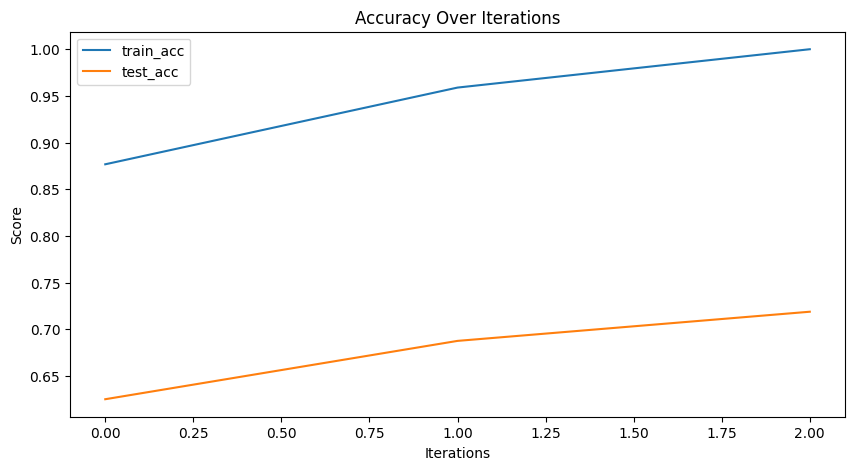
\includegraphics[width=\linewidth]{figs/active_learning.png}
    \caption{Active learning cycle through two iterations.}
    \label{fig:c4:active_learning}
  \end{figure}

A abordagem de active learning é aplicada para melhorar iterativamente o modelo, adicionando exemplos novos e informativos ao conjunto de treinamento. A modesta melhoria na precisão dos testes mostra que a aprendizagem activa está a contribuir para um melhor desempenho do modelo. No entanto, a diferença entre a precisão do treino e do teste ainda é significativa, o que sugere que o modelo pode estar a sofrer de sobreajuste. Esta disparidade geralmente indica que o modelo está a aprender a memorizar os dados de treino, incluindo ruídos e detalhes não aplicáveis ​​a casos gerais. Para mitigar este problema, é necessário analisar o erro do modelo e identificar quais emoções não estão a ser corretamente identificadas e porquê. Além disso, é importante incluir mais exemplos que desafiem o modelo e o forcem a generalizar melhor. A implementação de técnicas como data augmentation, dropout e regularização também pode ajudar a evitar o sobreajuste e melhorar a generalização do modelo.


NEXT STEPS:
\begin{itemize}
    \item Analise de erro do modelo para identificar quais sao as emoções e o porque de não serem corretamente identificadas;
    \item Incluir mais exemplos que desafiem o modelo e o forcem a generalizar melhor;
    \item Implementar data augmentation para aumentar a diversidade dos dados de treino para evitar overfitting;
    \item Implementar métodos como dropout e regularização para evitar overfitting;
\end{itemize}